%!TEX program = xelatex
%!TEX encoding = UTF-8 Unicode
\documentclass{imcs}

\usepackage{graphicx}
\usepackage{hyperref}
\usepackage{enumitem}
\usepackage{listings}
\usepackage{color}

\lstset{
  tabsize=4,
  language=C++,
  captionpos=b,
  frame=lines,
  numbers=left,
  numberstyle=\tiny,
  numbersep=5pt,
  breaklines=true,
  showstringspaces=false,
  basicstyle=\ttfamily\footnotesize,
  keywordstyle=\color[rgb]{0,0,1},
  stringstyle=\color{red}
}

\usepackage{courier}
\usepackage{titlesec}
\usepackage{lscape}
\usepackage{placeins}
\usepackage{tabularx}
\usepackage[Q=yes]{examplep}
\def\labelitemi{--}
% \usepackage{biblatex}

% \renewcommand\multicitedelim{\addsemicolon\space}

\titleformat*{\section}{\LARGE\bfseries\sffamily}
\titleformat*{\subsection}{\Large\bfseries\sffamily}
\titleformat*{\subsubsection}{\large\bfseries\sffamily}
\titleformat*{\paragraph}{\large\bfseries\sffamily}
\titleformat*{\subparagraph}{\large\bfseries\sffamily}

\makeatletter
\let\old@itemize=\itemize
\def\itemize{\old@itemize
\setlength{\itemsep}{10pt}
\setlength{\parskip}{0pt}
\setlength{\leftskip}{0pt}
}
\makeatother

\makeatletter
\let\old@enumerate=\enumerate
\def\enumerate{\old@enumerate
\setlength{\itemsep}{10pt}
\setlength{\parskip}{0pt}
\setlength{\leftskip}{0pt}
}\makeatother

\bibliographystyle{ugost2008}

\begin{document}
\setcounter{page}{2}
\setcounter{tocdepth}{2}
\tableofcontents
\pagebreak

\section*{Аннотация}
\addcontentsline{toc}{section}{Аннотация}
В данной работе описываются понятия интерактивных задач по программированию и задач на разработку интеллектуальных агентов, функционирующих в многоагентной виртуальной среде. Основная часть работы заключается в выявлении требований, предъявляемых к системе автоматической проверки решений задач по программированию "<CATS"> и доработке этой системы для эффективной поддержки новых классов задач.

\pagebreak

\section{Введение}
\subsection{Глоссарий}
\textbf{Интеллектуальный агент} — автономная сущность, получающая информацию о внешней среде и осуществляющая влияние на внешнюю среду, при этом их реакция рациональна в том смысле, что их действия содействуют достижению определенных параметров.

\textbf{Мультиплексирование} — объединение нескольких потоков данных в один.

\textbf{Поток данных} (англ. stream) в программировании — абстракция, используемая для чтения или записи файлов, сокетов и т. п. в единой манере. Потоки являются удобным унифицированным программным интерфейсом для чтения или записи файлов (в том числе специальных и, в частности, связанных с устройствами), сокетов и передачи данных между процессами. Поддержка потоков включена в большинство языков программирования и во все современные операционные системы. При запуске процесса ему предоставляются предопределённые стандартные потоки.

\textbf{Поток выполнения} (тред; от англ. thread — нить) — наименьшая единица обработки, исполнение которой может быть назначено ядром операционной системы. Реализация потоков выполнения и процессов в разных операционных системах отличается друг от друга, но в большинстве случаев поток выполнения находится внутри процесса. Несколько потоков выполнения могут существовать в рамках одного и того же процесса и совместно использовать ресурсы, такие как память, тогда как процессы не разделяют этих ресурсов. В частности, потоки выполнения разделяют инструкции процесса.

\textbf{Стандартные потоки ввода-вывода} — потоки процесса, имеющие номер (дескриптор), зарезервированный для выполнения некоторых "<стандартных"> функций. Как правило (хотя и не обязательно), эти дескрипторы открыты уже в момент запуска задачи (исполняемого файла). В число стандартных потоков входят: стандартный ввод (STDIN), стандартный вывод (STDOUT), стандартный вывод ошибок (STDERR).

\textbf{Controller (контроллер)} — программа, предоставляющая виртуальную среду для интеллектуальных агентов и контролирующая их действия, запущенная с помощью Spawner. Используется в многоагентных задачах.

\textbf{Control режим} — режим работы Spawner, если присутствует хотя бы  один контроллер.

\textbf{Interactor (интерактор)} — программа, выполняющая роль контроллера в интерактивных задачах. От интерактора не требуется управление программой-решением через Spawner, в отличии от контроллера.

\textbf{Normal (нормал)} — программа, выполняющая роль интеллектуального агента и запущенная с помощью Spawner.

\textbf{Pipe (пайп)} — объект операционной системы, посредством которого происходит реализация передачи данных по стандартным потокам ввода-вывода.

\textbf{Spawner} — программа, осуществляющая контролируемое исполнение произвольных программ, используемая в CATS.


\subsection{Описание предметной области}
\subsubsection{Соревнования по программированию}
На сегодняшний день в России и мире проводится множество соревнований по программированию, включая известный командный чемпионат мира по программированию среди студентов высших учебных заведений АСМ~ICPC~\cite{acm}, а так же школьные олимпиады по информатике. Подобные соревнования получили широкое распространение и помогают относительно объективно оценить уровень знаний и умений участников в области программирования~\cite{prog_challenges}. В рамках соревнований участникам предлагается набор задач, который они должны решить за определенное время, не выходя за заданные условиями задач и соревнований ограничения. Каждому участнику или команде участников предоставляется компьютер с предустановленным набором программного обеспечения, позволяющей сразу же приступить к решению задач. Некоторые соревнования допускают удалённое участие, а так же позволяют пользоваться системой автоматической проверки решений задач вне турниров — для тренировки.

При проведении соревнования по программированию, от организатора требуется разработать пакет заданий, состоящий из условий, набора тестов и эталонного решения для каждой задачи. Когда участник разработал программу и считает, что она удовлетворяет условиям задачи, он предоставляет данное решение для проверки организаторам, где, в свою очередь, проходит тестирование и сравнение результата работы программы участника с результатами работы эталонного решения. После этого делается вывод о корректности предложенного на проверку решения.

Для упрощения проведения соревнований используются системы автоматической проверки решений задач по программированию. Такие системы предоставляют интерфейсы для регистрации в турнире, получения условий, отправки условий, слежения за ходом турнира и автоматически проводят тестирование решений. Стоит заметить, что такие системы могут использоваться для автоматизации учебного процесса в дисциплинах информатики. Такая практика успешно применяется на кафедре информатики, математического и компьютерного моделирования ШЕН ДВФУ.

Последние годы в соревнования Всероссийской олимпиады школьников по информатике\cite{vseros} наблюдается появление нового вида задач — основанных на игровой стратегии\cite{elizarov}. Задачи данного вида далее будем называть интерактивными задачами.

\subsubsection{Соревнования Искусственного Интеллекта}
\label{ai_contest_intro}
Соревнование ИИ — мероприятие, посвящённое одновременному взаимодействию пользовательских программ, выполняющих роль интеллектуальных агентов в некоторой многоагентной среде. Среда может быть как реальной — например соревнования роботов, так и виртуальной, предоставляемой некоторым программным обеспечением. В данной работе нас интересует только последний случай. Данное взаимодействие осуществляется с целью выявления победителя — агента, который лучше остальных ведёт себя в данной среде, согласно условиям задачи, которая может не иметь объективно лучшего решения или же данное решение не может быть найдено за приемлемое время.

Сложность таких симуляций, обусловленная протяжённостью во времени в смысле пошагового выполнения и одновременного взаимодействия более одного агента, порождает необходимость использования программ визуализаторов хода турнира, для наглядности происходящего. На скриншотах ниже представлены примеры визуализаторов некоторых существующих популярных турниров ИИ.

Задачи, ставящиеся на таких соревнованиях будем называть интерактивными многоагентными, или просто многоагентными.

На рис.~\ref{robocode_screenshot} представлен визуализатор соревнования Robocode — в ходе которого на поле соревнуются танки. Задача каждого танка - выжить и уничтожить как можно больше противников. Каждый танк — управляется программой-агентом. На рис.\ref{warlight_screenshot} представлен визуализатор некоторого стратегического соревнования, заключающегося в пошаговом захвате территории. Некоторые системы предоставляют более одного типа соревнований и возможность разрабатывать программу-агент в веб-браузере Рис.~\ref{codingame_screenshot}.

\begin{figure}[htb]
\centering
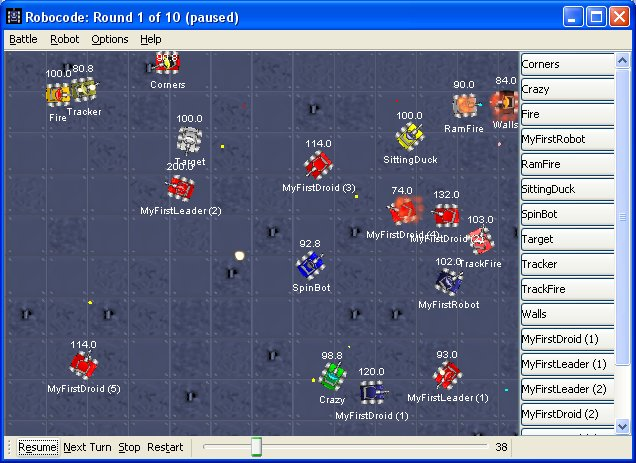
\includegraphics[width=\textwidth,keepaspectratio]{./img/robocode.jpg}
\caption{Robocode}
\label{robocode_screenshot}
\end{figure}

\begin{figure}[htb]
\centering
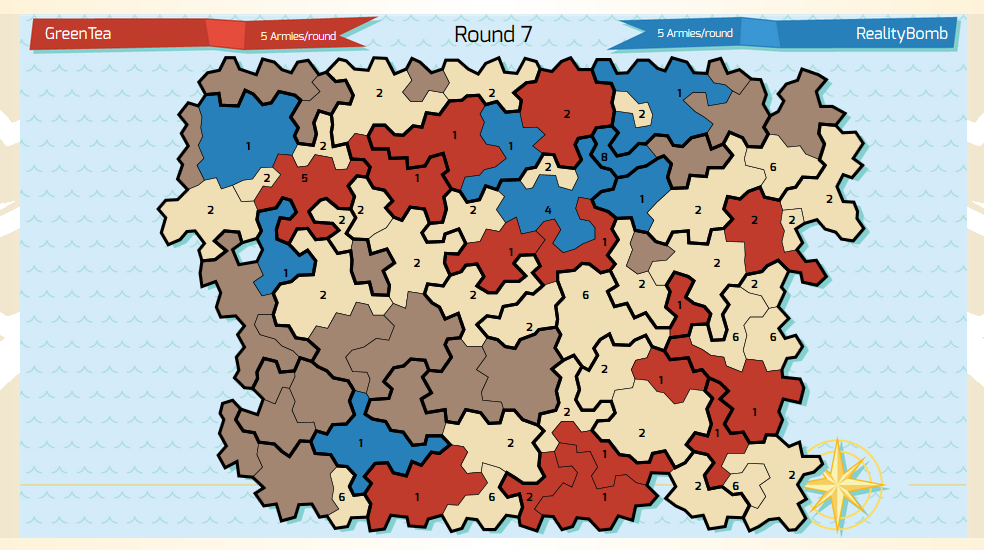
\includegraphics[width=\textwidth,keepaspectratio]{./img/warlight.png}
\caption{Warlight}
\label{warlight_screenshot}
\end{figure}

\begin{figure}[htb]
\centering
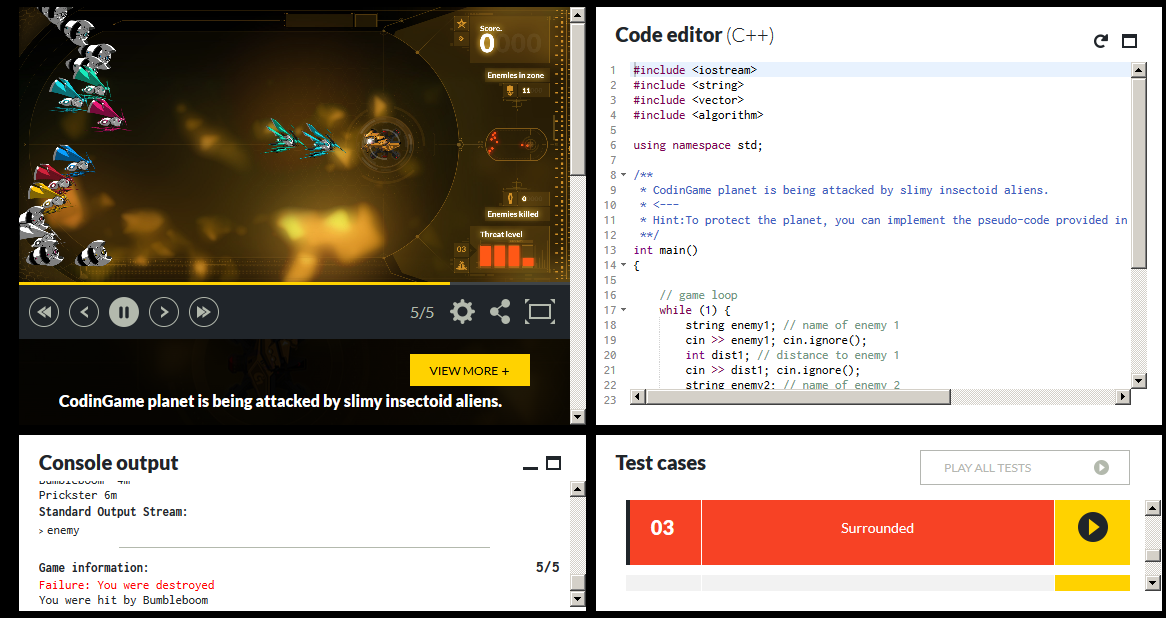
\includegraphics[width=\textwidth,keepaspectratio]{./img/codingame.png}
\caption{codingame.com}
\label{codingame_screenshot}
\end{figure}
\FloatBarrier

\subsubsection{Система CATS}
\FloatBarrier
\begin{figure}[htb]
\centering
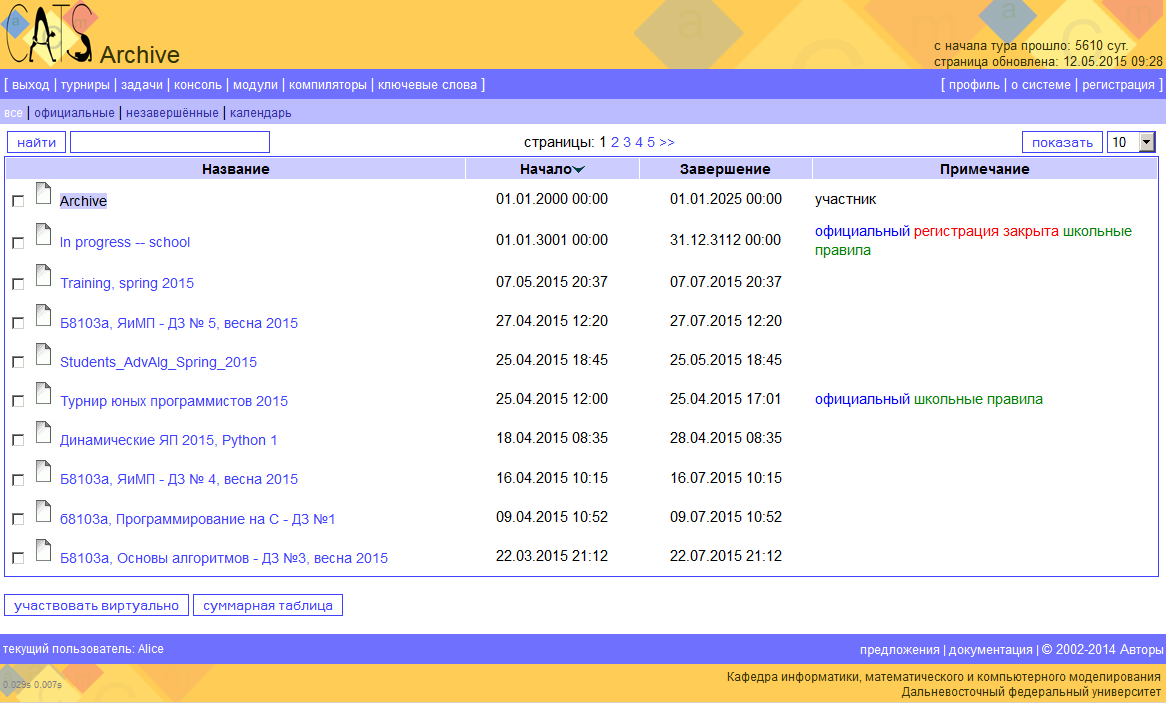
\includegraphics[width=\textwidth,keepaspectratio]{./img/cats_screenshot.png}
\caption{Веб-интерфейс системы}
\label{cats_screenshot}
\end{figure}

Одной из систем автоматизации организации соревнований по программированию является CATS~\cite{cats,rozhkov}~(Рис.~\ref{cats_screenshot}).
Система разрабатывалась на базе ДВФУ и успешно применяется при проведении соревнований начиная от школьных олимпиад и заканчивая четвертьфиналом чемпионата мира по программированию ACM ICPC.
История системы начинается с 2002 года и продолжается до сих пор.
За это время на базе CATS было проведено огромное количество соревнований, система неоднократно улучшалась и дополнялась~\cite{rozhkov,matvienko,konovalova,perepechin,tuphanov,khrapchenkov}.

CATS включает в себя такие компоненты как веб-интерфейс — cats-main, базу данных, компонент тестирования решений — cats-judge~\cite{rozhkov}, а так же компонент контролируемого исполнения программ Spawner (подробнее см. раздел Архитектура).

\paragraph{Веб-интерфейс} предоставляет возможность участвовать в доступных турнирах, просматривать задачи, отправлять соответствующие решения, выполненные в разрешенных системой (турниром) средах разработки, следить за ходом их тестирования, следить за ходом турнира и др. Для организаторов, в свою очередь, веб-интерфейс позволяет создавать турниры, добавлять в них задачи, следить за ходом турнира и др.

\paragraph{База данных} обеспечивает связь между веб интерфейсом и компонентом cats-judge, а так же хранит информацию о существующих в системе турнирах, участниках, задачах, решениях и пр.

Веб интерфейс и база данных являются кросс-платформенными составляющими системы и могут быть установлены на компьютеры под управлением различных операционных систем.

\paragraph{Компонент тестирования решений} отвечает за контролируемый запуск и тестирование программ решений участников. Во время исполнения программ от judge требуется чтобы они не нарушали набора ограничений на системные ресурсы, наборы правил безопасности, а в случае некорректного хода работы — информация о произошедших ошибках должна быть корректно обработана и учтена. После чего результаты о ходе тестирования и запуска решения участника отправляются в базу данных.

\paragraph{Компонент контролируемого исполнения} используется при тестирования решений. Предоставляет обеспечение безопасности, управление вводом/выводом и контроль за потребляемыми программой ресурсами, такими как память, время. Для задачи контролируемого исполнения в cats-judge используется компонент Spawner\cite{prototype}, представляющий собой отдельный программный продукт абстрагированный от предметной области спортивного программирования. Большая часть изменений вносимых в систему CATS в рамках данной работы касается непосредственно компонента Spawner.

Компонент Spawner имеет необходимый для поддержки интерактивных задач функционал, но поддержка данного типа задач не реализована в других компонентах CATS. В случае многоагентных задач необходима доработка компонента Spawner.

\subsubsection{Задачи}
Рассмотрим разницу между стандартными, интерактивными и многоагентными задачами в смысле потоков обмена данными и количества участников обмена данными в контексте CATS. На иллюстрациях ниже Н.П. — нормальная программа (решение стандартной или интерактивной задачи, либо интеллектуальный агент), У.П. — управляющая программа (интерактор или контроллер).

\begin{figure}[htb]
\centering
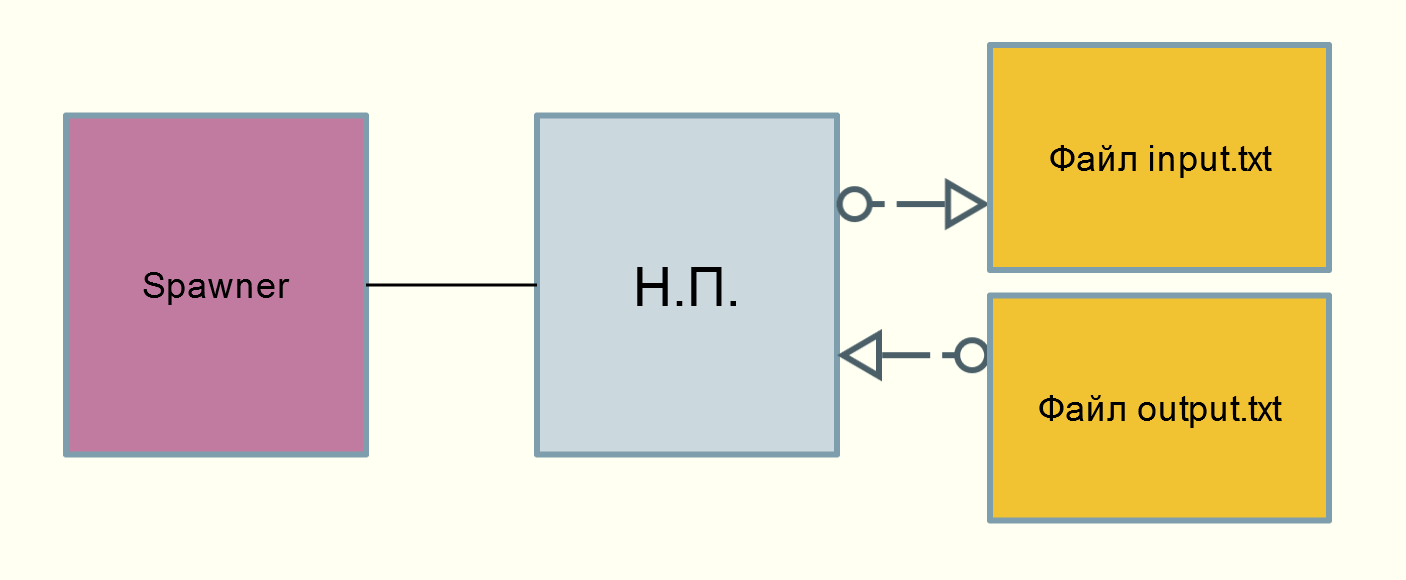
\includegraphics[width=\textwidth,keepaspectratio]{./img/normal_data_flow.png}
\caption{Потоки данных в стандартной задаче}
\label{normal_problem_flow}
\end{figure}

\FloatBarrier

Последовательность действия для проверки стандартной задачи включает в себя взаимодействие тестирующей системы и решения задачи (рис. \ref{normal_problem_flow}). Входные и выходные данные чаще всего передаются через файлы, указанные в условиях задачи или через стандартные потоки STDIN, STDOUT.

\FloatBarrier

\begin{figure}[htb]
\centering
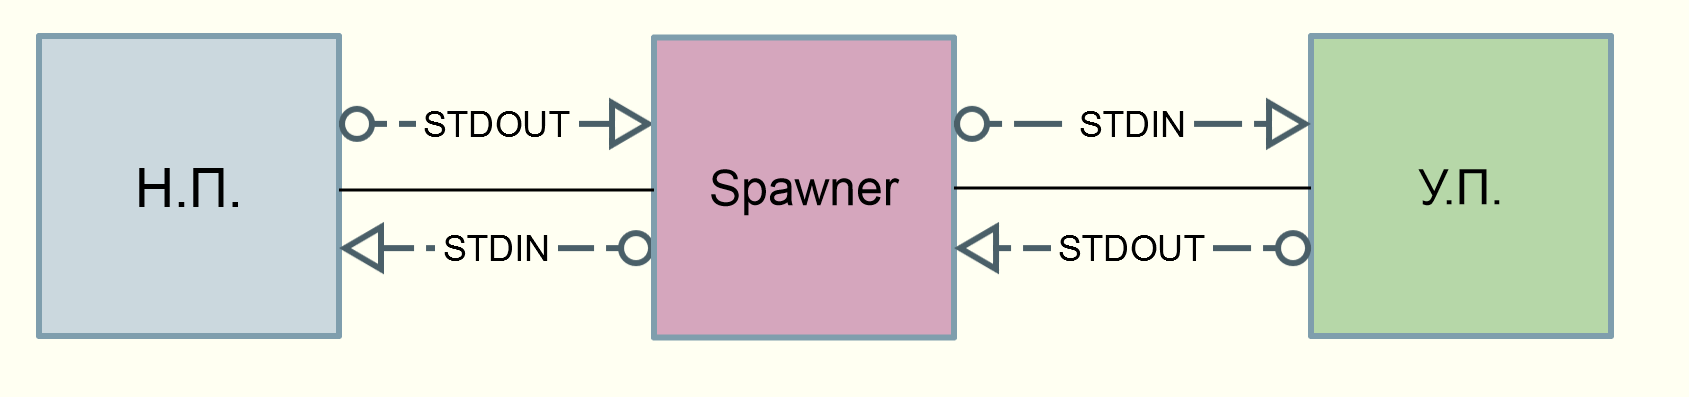
\includegraphics[width=\textwidth,keepaspectratio]{./img/interactive_data_flow.png}
\caption{Потоки данных в интерактивной задаче}
\label{interactive_problem_flow}
\end{figure}

\FloatBarrier

При использовании игровой стратегии, проверка решения рассматривается как игра двух противников — тестирующей системы (интерактор) и тестируемой программы (решение участника). Первый ход осуществляет тестирующая система (проверяющая программа). Далее ход переходит к тестируемой программе. Она запускается на входных данных, подготовленных тестирующей системой, и выдает некоторый результат. Ход вновь получает тестирующая система. Она анализирует результат, полученный тестируемой программой. На основе результатов анализа принимается решение о продолжении тестирования. Если тестирование продолжается, то проверяющая система подготавливает новый набор входных данных,  при этом может быть использована информация , полученная от тестируемой программы, на предыдущих шагах. После чего ход снова передается тестируемой программе, и так далее (см. Рис.~\ref{interactive_problem_flow}). \cite{elizarov}

\FloatBarrier

\begin{figure}[htb]
\centering
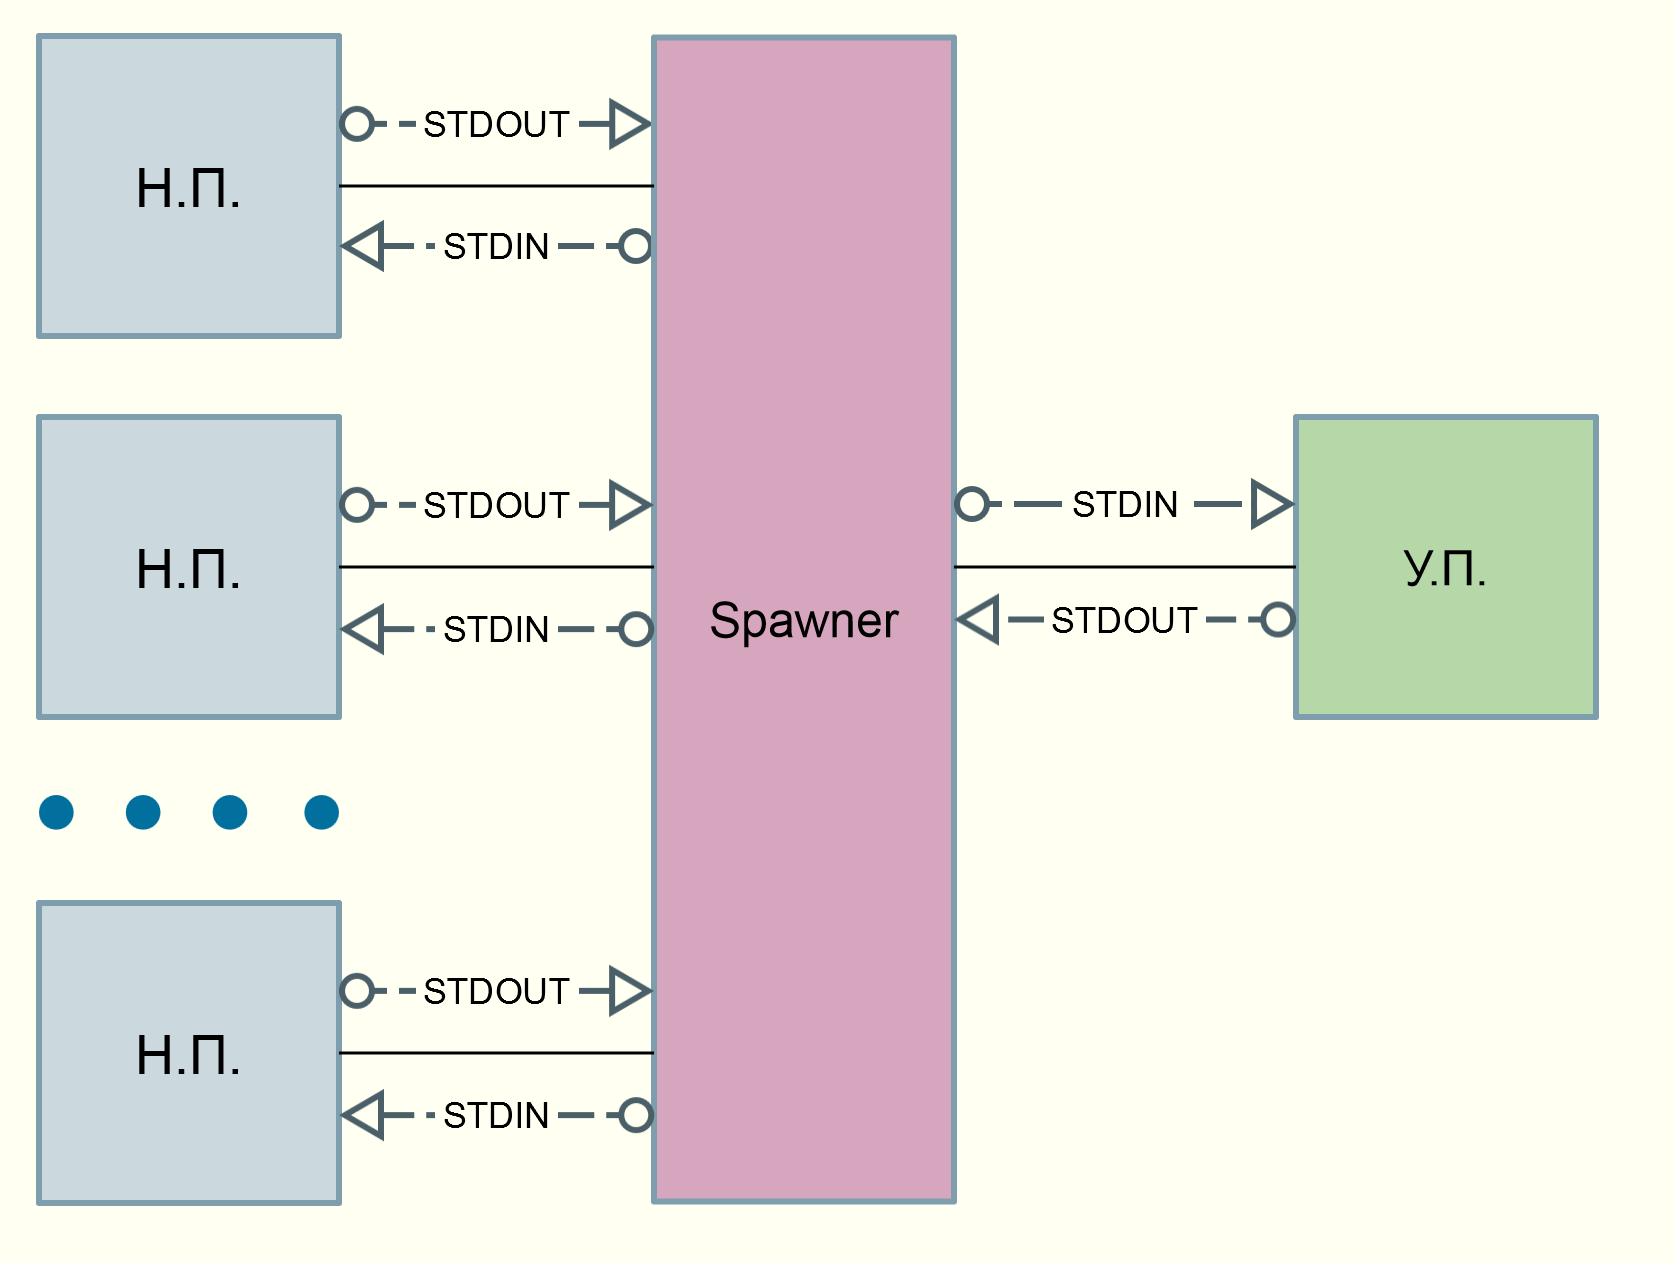
\includegraphics[width=\textwidth,keepaspectratio]{./img/multiagent_data_flow.png}
\caption{Потоки обмена данных в многоагентных задачах}
\label{multiagent_data_flow}
\end{figure}

\FloatBarrier

В случае многоагентных задач увеличивается количество одновременно взаимодействующих программ и у тестирующей программы (контроллера) появляется необходимость управлять исполнением нормальных программ через Spawner. При этом взаимодействие с контроллером по прежнему осуществляется через два стандартных потока ввода-вывода, что наталкивает на мысль о необходимости мультиплексирования каналов связи по некоторому протоколу. (рис. \ref{multiagent_data_flow}).

\FloatBarrier

\subsection{Неформальная постановка задачи}

Целью данной работы ставится расширение поддерживаемых CATS классов задач:
\begin{itemize}
  \item Использование интерактивных задач в CATS
  \item Расширение Spawner для поддержки многоагентных задач
\end{itemize}

\subsection{Обзор существующих методов решения}

\subsubsection{Системы организации соревнований}
В рамках данной работы было проведено изучение подобных систем организации соревнований по программированию.

\paragraph{ejudge} — это система для проведения различных мероприятий, в которых необходима автоматическая проверка программ. Система может применяться и применяется для проведения олимпиад, поддержки учебных курсов и т.д. Система предоставляет веб-интерфейс администратора и участника турнира, а так же доступ к серверам турниров из командной строки. \cite{ejudge}

\paragraph{PCMS2 (Programming Contest Management System)} — Используется во время проведения Всероссийского этапа ACM ICPC. \cite{pcms2}

\paragraph{Contester} — это система для проведения турниров и индивидуального решения задач по олимпиадному программированию (спортивному программированию). Система содержит условия задач - от легких до олимпиадных - и возможность проверки решений на большинстве современных языков: C++, Object Pascal, Java и языках .NET: C\#, J\# и Visual Basic.

Contester работает на Windows и на Linux. Язык реализации Delphi/freepascal. Представляет собой полноценную систему организации соревнований готовую к запуску с момента установки и распространяется в виде установочного файла или архива, в зависимости от операционной системы. \cite{contester}

\paragraph{PC$^2$ (Programming Contest Control System)} — система разработанная в Калифорнийском Государственном Университете Sacramento (CSUS) в поддержку соревнований по программированию, проводимых ACM и, в частности, ACM International Collegiate Programming Contest (ICPC) и его региональных этапов. \cite{pccs}

\paragraph{DOMjudge} — автоматизированная тестирующая система, для проведения соревнований по программированию, подобных ACM ICPC. Основной упор сделан на удобство использования и безопасность. Система применялась во многих соревнованиях, распространяется свободно на условиях открытого ПО.
Для контроля исполнения используется набор небольших консольных утилит. \cite{domjudge}

\paragraph{dudge} — это универсальная система для проведения олимпиад по программированию и другим предметам, написанная на Java и J2EE с использованием СУБД PostgresSQL и распространяющаяся по лицензии GPL. \cite{dudge}

\begin{landscape}
\begin{table}[h!]
\begin{center}
\begin{tabularx}{25cm}{|X|X|X|X|X|X|X|}
\hline
Название & Интерактивные задачи & Соревнования ИИ & Лицензия & Последняя версия \\ \hline
ejudge & Да & Нет & GPL & 3.3.0, 15.01.2014 \\ \hline
PCMS2 & Да & Нет & Проприетарная & 2, 17.11.2004 \\ \hline
Contester & Нет & Нет & Проприетарная & 2.4, 07.11.2010 \\ \hline
PC$^2$ & Да & Нет & Проприетарная & 9.2.4, 20.09.2014 \\ \hline
DOMjudge & Да & Нет & GPL & 4.0.4, 27.10.2014 \\ \hline
dudge & Нет & Нет & GPL & GIT-master \\ \hline
\end{tabularx}
\caption{Сравнение доступных систем контроля исполнения программ}\label{tab:wsi_diff_rel}
\end{center}
\end{table}
\end{landscape}

\subsubsection{Системы искусственного интеллекта}
Скриншоты некоторых таких системы были приведены в \ref{ai_contest_intro}. Было рассмотрено несколько таких систем. В результате было выявлено, что подавляющее их большинство (например Robocode\cite{robocode}, Rock Paper Scissors\cite{rockpaperscissors}, Vindinium\cite{vindinium}, Code Cup\cite{codecup}, Google AI Contests) специализированно для одной конкретной задачи. Те из них, что поддерживают множество задач (Hacker Rank\cite{hackerrank}, Coding Game\cite{codingame}) не предоставляют пользователям возможность разработки задач и являются закрытыми, что затруднило подробный анализ.

\subsubsection{Системы контролируемого исполнения}
Средства контролируемого исполнения применяются во многих областях, например Online IDE, Тестирующие системы, антивирусы, Continuous Integration. В рамках данной работы нас интересует поддержка многозадачности в таких системах, что означает не только возможность одновременно запускать несколько процессов но и предоставить возможность некоторым процессам взаимодействовать с системой контролируемого исполнения и другими процессами, а так же предоставляют возможность одним контролируемым процессам управлять выполнением других.

Существующие средства не предоставляют широких возможностей настройки взаимодействия процессов через стандартные потоки, а так же не предоставляют интерфейса контроля других процессов.

Среди прочих стоит выделить программный комплекс Docker, который позволяет настраивать отображение портов контейнеров, в которых запускаются процессы, связывая их и тем самым позволяя общаться друг с другом. \cite{docker}. Данный подход обеспечивает только обмен данными между процессами, при чём посредством сетевого взаимодействия, что нас не устраивает.

\subsubsection{Вывод}

Большинство систем автоматизации проведения соревнований и тестирования решений задач имеют поддержку интерактивных задач, но не было обнаружено ни одной, имеющей встроенную возможность проведения соревнований ИИ. Добавление в CATS поддержки интерактивных задач позволит расширить класс поддерживаемых задач и использовать в CATS интерактивные задачи с проводимых в других системах турниров.

Существующие системы соревнований ИИ узконаправленны или предоставляются на платной основе как сервис, без возможности самостоятельной разработки новых задач.

Требуется значительная доработка модуля Spawner для того чтобы интеграция турниров ИИ в CATS стала возможной.

\section{Требования к окружению}
\subsection{Требования к программному и аппаратному обеспечению}
Для сборки проекта Spawner требуется система cmake версии не менее 2.8. Компиляция Spawner требует наличие компилятора языка C++11, поддерживаемого системой cmake. Был протестирован компилятор входящий в состав Visual Studio 2013, а так же GCC 4.9. Spawner функционирует только на системах семейства Windows, начиная с Windows XP. Полная поддержка доступна начиная с Windows Vista, что связанно с использованием функции WinAPI CancelSynchronousIo, необходимой для отмены синхронных операций ввода-вывода в пределах потока.

Требования к остальным компонентам системы рассмотрены в \cite{rozhkov}.

\section{Архитектура системы}

CATS является аппаратно-программным комплексом, состоящим из нескольких компонент: веб-интерфейс, база данных, тестирующий компонент cats-judge и модуль контроллируемого исполнения Spawner.

\begin{figure}[htb]
\centering
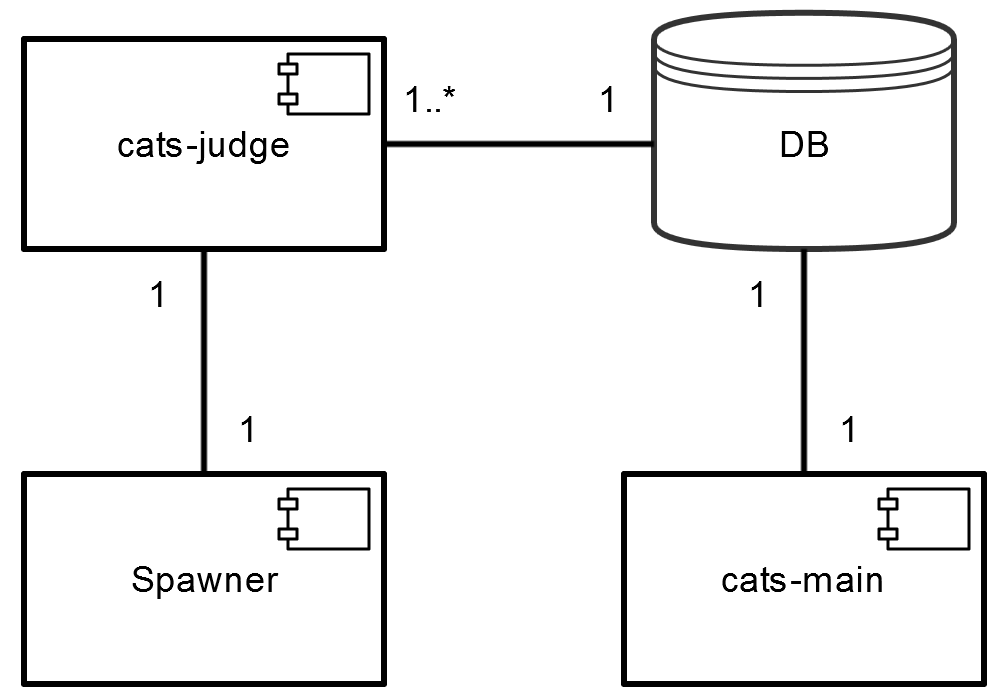
\includegraphics[width=\textwidth,keepaspectratio]{./img/cats.png}
\caption{Компоненты CATS}
\label{cats}
\end{figure}

\FloatBarrier

\subsubsection{Веб-интерфейс}
Веб-интерфейс~\cite{rozhkov} является кросс-платформенной частью системы. Веб сервер может быть запущен практически на любой системе.
Фактически, с помощью веб-интерфейса осуществляется управление содержимым базы данных.

\subsubsection{База данных}
\FloatBarrier
В базе данных~\cite{rozhkov} системы хранятся данные о проводимых турнирах, пакеты задач, исходный код, информация об участниках, их попытках, а так же информация по средам разработки.
Однако привязка модуля judge к какому-либо виду базы данных усложняет его развертывание на конечной машине.

\FloatBarrier
\subsubsection{Компонент cats-judge}
\FloatBarrier
cats-judge\cite{rozhkov} содержит загруженный кэш задач, кэш попыток, различные конфигурационные файлы и модуль Spawner.

Обычно, для сокращения нагрузки одновременно запущено несколько компьютеров с judge. Они подключаются к базе данных и распределяют задачи на исполнение между собой.

\FloatBarrier
В случае отсутствия задачи в кэше происходит загрузка из базы данных, генерация тестов и т.д.

В общем случае коммуникация между модулями проходит в следующем порядке:

\FloatBarrier
\begin{figure}[htb]
\centering
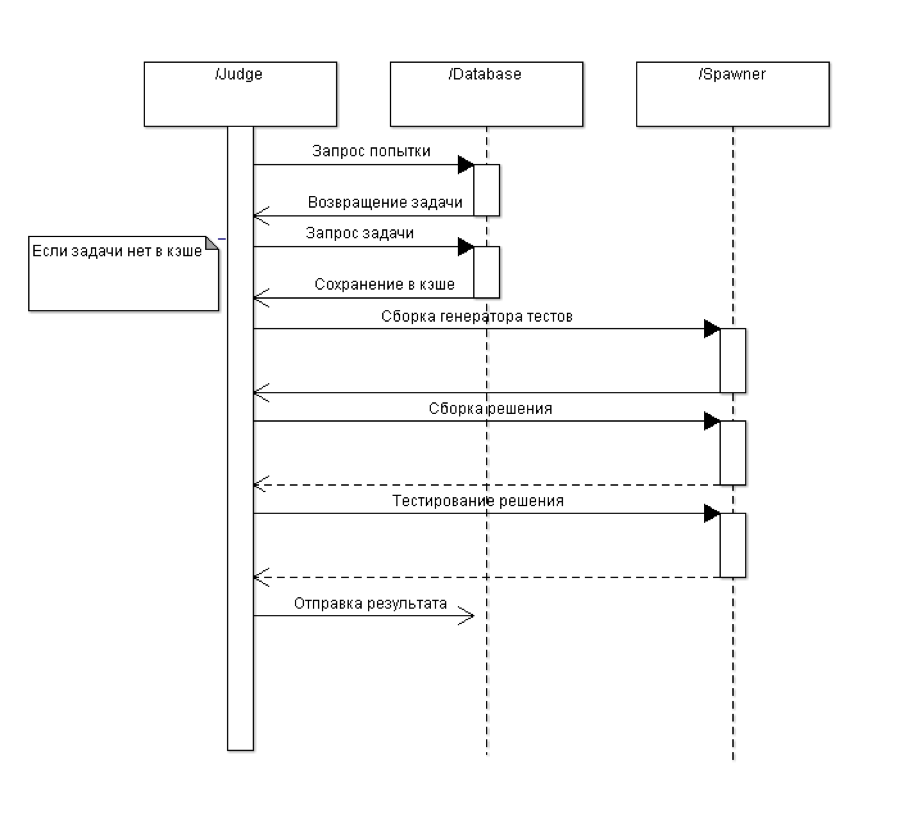
\includegraphics{./img/judgeinteraction.png}
\caption{Схема работы cats-judge}
\label{judgeinteraction}
\end{figure}

\FloatBarrier
\subsubsection{Модуль Spawner}

Во время проведения тестирования требуется создать для программы изолированную среду и задать необходимые ограничения на ресурсы. Так же в случае некорректного хода исполнения тестируемой программы требуется определить характер и возможную причину ошибок и должным образом отреагировать на это. Эти задачи решает компонент Spawner.

В данной работе важно, что Spawner так же позволяет связывать друг с другом стандартные потоки запускаемых процессов. На рис. \ref{data_flow} изображена схема связи стандартных потоков ввода-вывода для случая двух процессов, с акцентом на внутреннее устройства. Такого типа связи могут быть установленны между любыми двумя стандартными потоками ввода и вывода любых процессов, одновременно находящихся в контролируемом исполнении. Таким образом схема может быть расширена на произвольное количество процессов. Каждому входному и каждому выходному потоку соответствует поток исполнения Spawner. Поток чтения следит за появлением данных в STDOUT пайпе и перенаправляет их в своё множество буферов. Это множество буферов может пересекаться с множеством буферов потока записи, так как каждый буфер связывает ровно два потока. Поток записи следит за появлением данных в своих буферах и перенаправляет их в STDIN пайп.

\begin{figure}[htb]
\centering
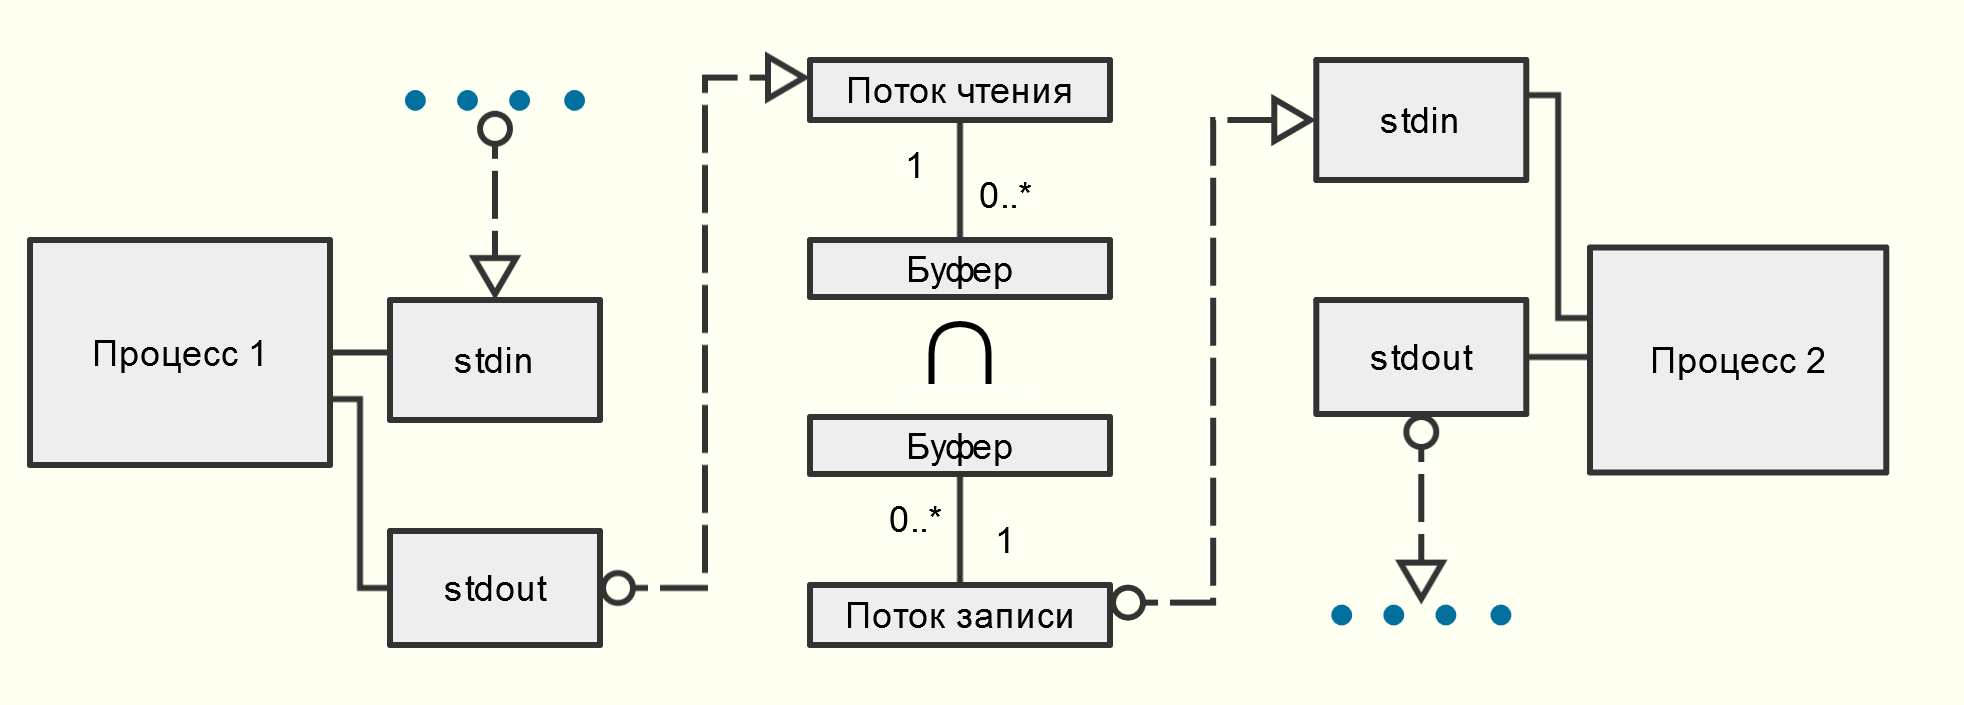
\includegraphics[width=\textwidth,keepaspectratio]{./img/data_flow.png}
\caption{Связь стандартных потоков}
\label{data_flow}
\end{figure}

\FloatBarrier

\section{Спецификация данных}
\subsection{Аргументы командной строки Spawner}
Аргументы командной строки Spawner подробно описаны в \cite{khrapchenkov}. В рамках данной работы стоит рассмотреть способ запуска нескольких процессов, а так же формат связи потоков ввода-вывода запускаемых процессов.

\begin{itemize}
\item { необходимо указать последовательность символов — разделитель, которая будет отделять секции аргументов командной строки для каждого запускаемого процесса. Это осуществляется с помощью ключа --separator:
\begin{lstlisting}
sp.exe --separator=//
--// p1.exe
--// p2.exe
--// p3.exe
--// p4.exe
\end{lstlisting}
Таким образом будет запущено 4 процесса. Для настройки параметров процесса нужные флаги должны помещаться в соответствующую секцию.
}
\item { для того, чтобы осуществить связь потоков ввода вывода необходимо использовать флаги --in=<name> для STDIN и --out=<name> для STDOUT, где <name> имеет формат *<число>.stdin или *<число>.stdout, что позволяет сослаться на соответствующие потоки запускаемого процесса с индексом <число>. Процессы нумеруются в порядке их передачи Spawner, начиная с 0. Так же может быть указано значение --in=std или --out=std, что осуществляет перенаправление на стандартный ввод/вывод. Следующая командная строка связывает STDOUT контроллера с STDIN каждого нормала и STDIN контроллера с STDOUT каждого нормала:
\begin{lstlisting}
sp.exe --separator=//
--// controller.exe
--// --in=*0.stdout --out=*0.stdin normal-1.exe
--// --in=*0.stdout --out=*0.stdin normal-2.exe
--// --in=*0.stdout --out=*0.stdin normal-3.exe
\end{lstlisting}
}
\item { для того чтобы пометить запускаемый процесс как контроллер требуется передать ключ --controller:}
\begin{lstlisting}
sp.exe --controller controller.exe
\end{lstlisting}
\end{itemize}

\subsection{Протокол обмена данными}
Рассмотрим отличие обычных задач, от интерактивных и многоагентных.

\begin{figure}[htb]
\centering
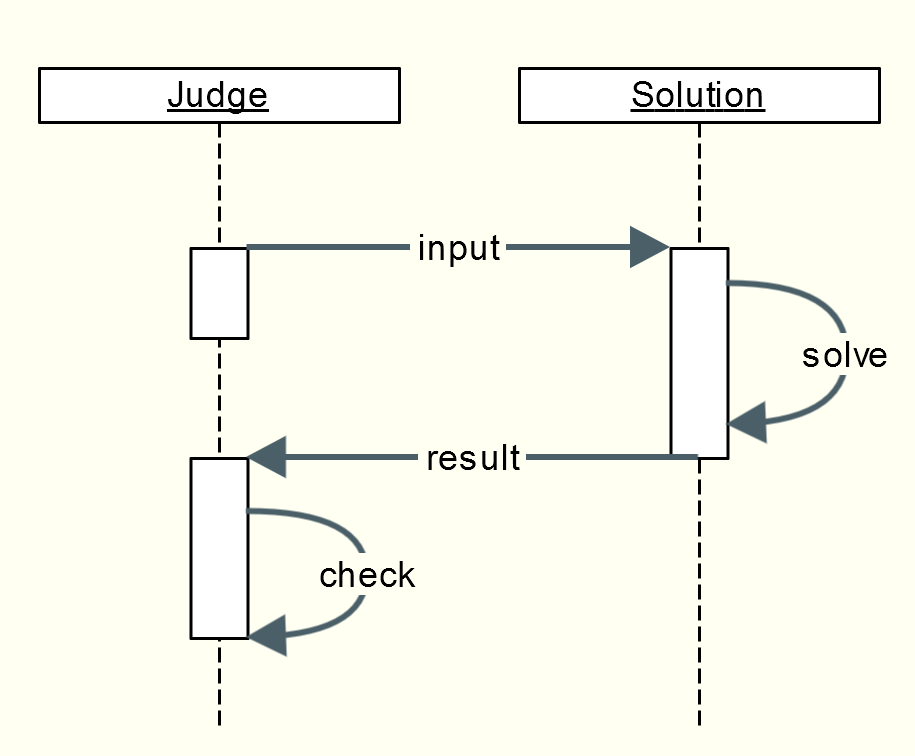
\includegraphics[width=\textwidth,keepaspectratio]{./img/normal_problem.png}
\caption{Последовательность проверки обычной задачи}
\label{normal_problem}
\end{figure}

\FloatBarrier

Последовательность действия для проверки обычной задачи включает в себя взаимодействие judge и решения задачи (рис. \ref{normal_problem}).

\FloatBarrier

\begin{figure}[htb]
\centering
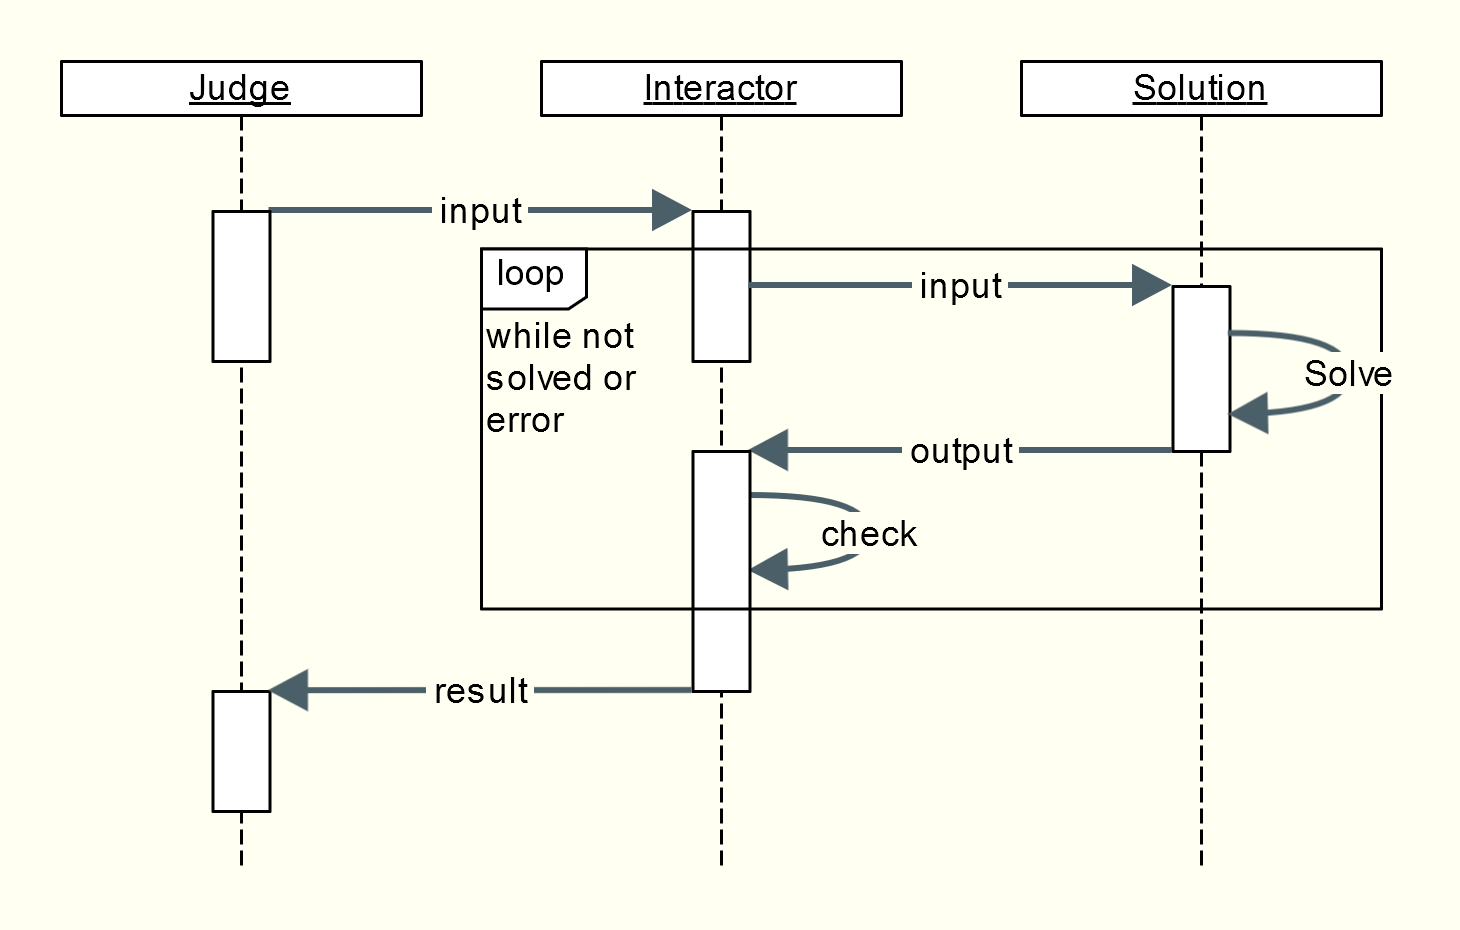
\includegraphics[width=\textwidth,keepaspectratio]{./img/interactive_problem.png}
\caption{Последовательность проверки интерактивной задачи}
\label{interactive_problem}
\end{figure}

\FloatBarrier

В случае же интерактивных задач появляется необходимость в дополнительной программе - интеракторе. Происходит обмен сообщениями между интерактором и решением в цикле (рис. \ref{interactive_problem}).

\FloatBarrier

\begin{figure}[htb]
\centering
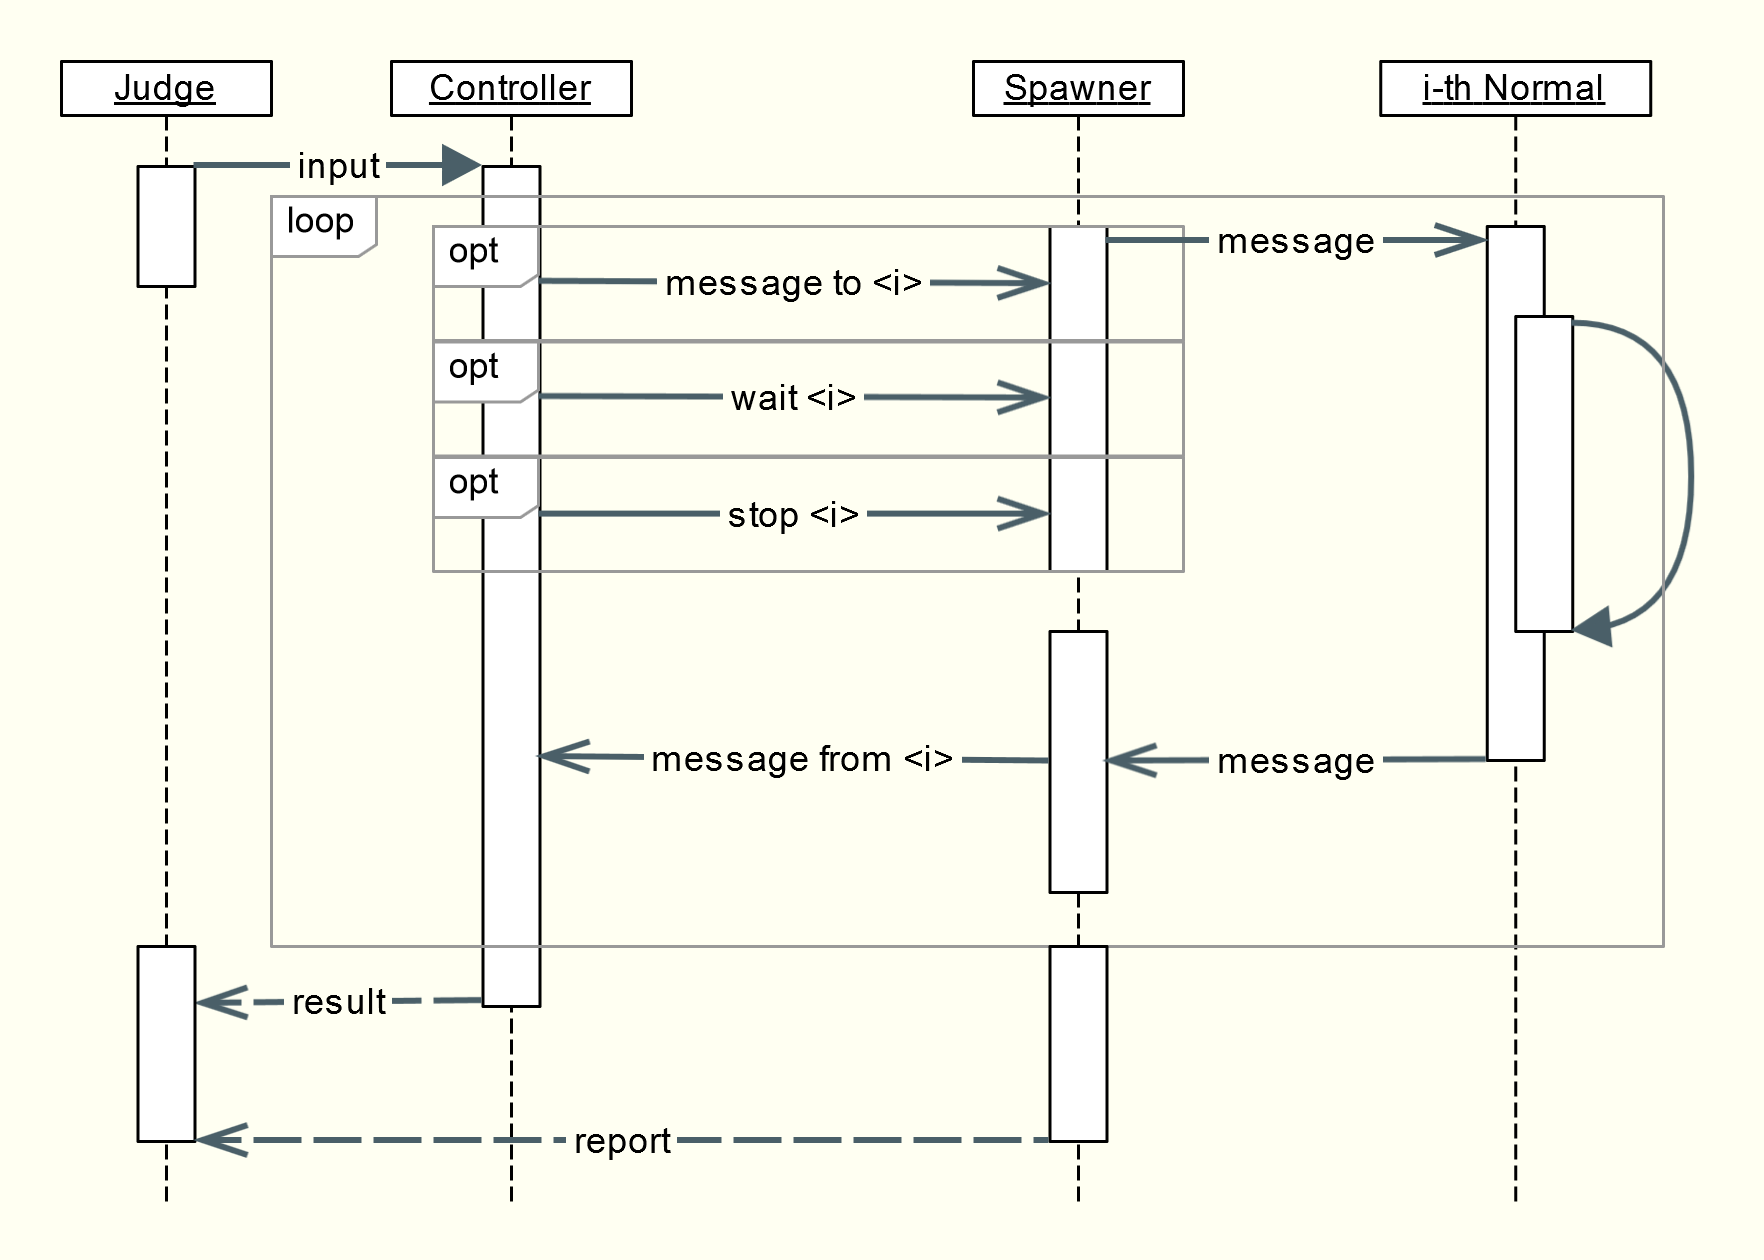
\includegraphics[width=\textwidth,keepaspectratio]{./img/ai_contest_problem.png}
\caption{Последовательность действия в режиме турнира ИИ}
\label{ai_contest_problem}
\end{figure}

\FloatBarrier

Для многоагентных задач взаимодействие со Spawner перестаёт быть прозрачным и учитывается тот факт, что одновременно происходит взаимодействие интерактора и нескольких решений задачи (рис. \ref{ai_contest_problem}).

\FloatBarrier

Данный протокол был разработан для мультиплексирования выходных потоков нескольких нормалов в один канал связи — стандартный входной поток контроллера, а так же демультиплексирования выходного потока контроллера во входные потоки нескольких нормалов, что позволяет контроллеру определить от какого нормала пришло сообщение, а так же доставить сообщение от контроллера указанному нормалу.

Целью данного протокола так же является возможность контроллера управлять выполнением нормалов — он может указать ожидание ввода от нормала, что выведет процесс нормала из suspended режима, а так же остановить процесс любого нормала, посредством отсылки Spawner специальных сообщений.

В контексте предметной области данный протокол будет использован для реализации поддержки многоагентных задач. Для интерактивных задач верным остаётся только необходимость сброса стандартного потока вывода, как для интерактора, так и для нормала, а так же тот факт, что разделителем сообщений является символ перевода строки.

\subsubsection{Схема запуска}
Контроллер и нормал запускаются с помощью Spawner, передаваемые в качестве аргументов командной строки. Предъявляются следующие требования:

\begin{itemize}
\item контроллер должен быть помечен флагом --controller.
\item контроллер должен быть единственным
\item наличие контроллера должно переводить spawner в режим управления
\item остальные требования применимы только в режиме управления
\item Количество нормалов должно быть передано контроллеру первым аргументом командной строки
\item stdin каждого нормала должен быть соединён с stdout контроллера с помощью --in=*0.stdout
\item stdout каждого нормала должен быть соединён с stdin контроллера с помощью --out=*0.stdin
\end{itemize}

Пример командной строки запуска:
\begin{lstlisting}
sp.exe --json -sr=report.json -hr=1 --separator=//
  --// --controller --out=std controller.exe 3
  --// --out=std --in=*0.stdout --out=*0.stdin normal-1.exe
  --// --out=std --in=*0.stdout --out=*0.stdin normal-2.exe
  --// --out=std --in=*0.stdout --out=*0.stdin normal-3.exe
\end{lstlisting}

\subsubsection{Правила Взаимодействия}

\begin{itemize}
\item все нормалы должны запускаться в приостановленном (suspended) состоянии
\item Spawner должен продолжать (resume) выполнение указанного нормала, в ответ на запрос ожидания данного нормала от контроллера
\item Spawner должен приостанавливать выполнение нормалов после получения от них сообщения, если контроллер ожидал ответа от данного нормала
\item контроллер может послать сообщение конкретному нормалу
\item контроллер может послать Spawner запрос на ожидание сообщения от конкретного нормала
\item нормал может послать сообщение контроллеру
\item контроллер может послать Spawner запрос на полную остановку указанного нормала
\item ограничения времени контроллера должны быть сброшены после каждого сообщения, посланного контроллером
\item ограничения времени нормала должны быть установленны в ответ на запрос ожидания данного нормала контроллером
\item ограничения времени нормала должны быть сброшены при отсылке нормалом сообщения
\end{itemize}

\subsubsection{Сообщения}
Сообщения имеют форму <заголовок><тело><перевод строки> Тело может состоять из любых символов кроме символов перевода строки или возврата каретки. Заголовок должен всегда кончаться символом \#. Перед символом \# может быть латинская буква, перед которой в свою очередь может быть целое число.

\begin{itemize}
\item контроллер и нормал должны отсылать сообщения через stdout
\item stdout должен быть сброшен (flushed) после отсылки сообщения
\item сообщения должны заканчиваться символом перевода строки
\end{itemize}

\subsubsection{Примеры сообщений}
Два сообщения:
\begin{lstlisting}
printf("First message\nSecond message\n");
fflush(stdout);
\end{lstlisting}

Одно сообщение:
\begin{lstlisting}
printf("\n");
fflush(stdout);
\end{lstlisting}

Забыт перевод строки:
\begin{lstlisting}
printf("foo");
fflush(stdout);
\end{lstlisting}

Не сброшен буфер:
\begin{lstlisting}
printf("foo\n");
\end{lstlisting}

\subsubsection{Сообщения контроллера}
Контроллер может отсылать два типа сообщений — сообщения для нормала и сообщения для Spawner.

При отсылке сообщений нормалу, контроллер обязан указать в заголовке сообщения индекс нормала, которому предназначено сообщение. Нормалы индексируются в порядке их передачи Spawner в качестве аргументов командной строки, начиная с единицы.

Например для такой схемы запуска:
\begin{lstlisting}
 sp.exe --separator=//
 --// --controller controller.exe 3
 --// --in=*0.stdout --out=*0.stdin normal-1.exe
 --// --in=*0.stdout --out=*0.stdin normal-2.exe
 --// --in=*0.stdout --out=*0.stdin normal-3.exe
\end{lstlisting}

Чтобы отослать сообщение "Foo" приложению normal-1.exe контроллер должен выполнить следующий код:
\begin{lstlisting}
printf("1#Foo\n");
fflush(stdout);
\end{lstlisting}

Если контроллер указывает неверный индекс, то Spawner обязан ответить контроллеру сообщением об ошибке:
\begin{lstlisting}
<i>I#\n
\end{lstlisting}

где \Q{<i>} — это индекс неверного normal.

Контроллер может сообщить Spawner об ожидании им ответа от конкретного нормала: <i>W\#<перевод строки>

Контроллер может запросить Spawner прекратить выполнение процесса указанного нормала с помощью сообщения <i>S\#. Spawner не должен сообщать об ошибке на запрос остановки, если индекс неверен.
Например чтобы запросить остановку нормала с индексом 4:
\begin{lstlisting}
printf('4S#\n');
fflush(stdout);
\end{lstlisting}

Сообщения отсылаемые по индексу 0 считаются сообщениями, отсылаемыми spawner. Дополнительный латинский символ может уточнить значение сообщения. Этот случай зарезервирован для последующих версий протокола.

\subsubsection{Сообщения нормала}
Spawner обязан дополнить слева сообщения normal его индексом и символом \# чтобы образовать заголовок сообщения, который будет разобран контроллером.

Например:
\begin{lstlisting}
// let this normal's index be 3
printf("12 45 56 65\n");
fflush(stdout);
// controller will get "3#12 45 56 65\n"
\end{lstlisting}

\subsection{Формат пакета задачи}
Описание конфигурации задачи представляет собой XML файл. Формат этого файла в полной мере описан в документации к CATS. \cite{catsprobformat}

В данной работе в рамках добавления поддержки интерактивных задач в формат заданий добавляется тэг Run для тэга верхнего уровня Problem. Данный тэг имеет атрибут method, принимающий значения interactive или default.

\begin{lstlisting}
<Run method="interactive" />
\end{lstlisting}

\subsection{Конфигурация модуля cats-judge}
Настойка доступных сред разработки и способов запуска для этих сред осуществляется с помощью XML файла config.xml находящегося в корневом каталоге cats-judge. Правила заполнения этого файла см. в \cite{rozhkov}. В данной работе в config.xml были добавлены следующие примитивы:

\begin{itemize}
\item{ run\_interactive - способ запуска с помощью Spawner в интерактивном режиме:
\begin{lstlisting}
<define name="#run_interactive" value="#spawner --separator=// -hr=1 --out=nul -wl=30 -tl=%time_limit -ml=%memory_limit -y=1 --// -sr=report.txt --in=*1.stdout --out=*1.stdin %interactor_name --// %deadline -sr= "/>
\end{lstlisting}
}
\item{ default\_interactor\_name - имя программы интерактора по-умолчанию:
\begin{lstlisting}
<define name="#default_interactor_name" value="Interact.exe" />
\end{lstlisting}
}
\item{ в каждую секцию среды разработки, поддерживающую интерактивные задачи должен быть добавлен атрибут run\_interactive:
\begin{lstlisting}
<!-- Cross-platform C/C++ compiler -->
<de
    code="101"
    compile='#spawner #gnu_cpp -O2 "%full_name" -o "%name.exe"'
    run='#run "%name.exe"'
    run_interactive='#run_interactive "%name.exe"'
    runfile='%name.exe'
    generate='#spawner%redir %limits "%name.exe" %args'
    check='#spawner %limits "%name.exe" %checker_args'/>
\end{lstlisting}
}
\item{ имя программы-интерактора по умолчанию может быть переопределено для среды разработки с помощью атрибута interactor\_name, например для Java:
\begin{lstlisting}
<!-- Java -->
<de
    code="401"
    compile='#spawner %comspec% /C ..\javac.cmd "%full_name"'
    run='#run "#java\java.exe" -Xss64m "%name"'
    interactor_name='"#java\java.exe" -Xss64m "Interact"'
    run_interactive='#run_interactive "#java\java.exe" -Xss64m "%name"'
    runfile='%name.class'
    generate='#spawner%redir %limits -wl:100 "#java\java.exe" -Xmx256m -Xss64m "%name" %args'
    check='#spawner %limits "#java\java.exe" -Xss64m "%name" %checker_args'/>
\end{lstlisting}
}
\end{itemize}


\section{Функциональные требования}

Для интерактивных задач требуется поддерживать тот же функционал CATS что и для обычных задач\cite{rozhkov}. Так как интерактивные задачи отличаются только методом запуска, то реализация этого функционала не потребует больших трудозатрат.

От компонента Spawner требуется:
\begin{itemize}
\item обеспечить возможность обменна данными между контроллером и нормалом посредством стандартных потоков ввода-вывода
\item предоставить контроллеру
\begin{itemize}
\item информацию о количестве нормалов в симуляции
\item возможность завершения указанного нормала
\item возможность определить индекс нормала, отправившего сообщение
\item возможность отсылать сообщение указанному нормалу
\end{itemize}
\item корректно обрабатывать ситуацию прекращения работы нормала и продолжения симуляции
\end{itemize}

\section{Проект}

Подробное описание устройства проекта может быть найдено в \cite{khrapchenkov}. В данном разделе будут рассмотрены внесённые изменения в различные модули, а так же описано и обосновано принятие некоторых решений.

\subsection{Средства реализации}
Для внесения изменений в компоненты cats-main и cats-judge использовался ЯП Perl, как основной язык системы. Изменения в Spawner вносились с использованием ЯП С++11. Выбор данного стандарта C++ обоснован тем фактом, что актуальные версии популярных компиляторов С++ почти в полной мере поддерживают данный стандарт, а его использование позволяет более выразительно писать код, что уменьшает время разработки, а так же улучшает читаемость кода.

Для обеспечения возможности вывода stacktrace использовалась сторонняя библиотека stackwalker\cite{stackwalker}.

\subsection{Интерактивные Задачи}

Для поддержки интерактивных задач добавлено понятие метода запуска. Данное поле было добавлено в БД в таблицу Problems, в класс Problem компонента cats-main. Парсер формата задачи в компоненты cats-main был доработан для поддержки формата задачи с учётом разбора метода запуска. В cats-judge потребовалось добавить выбор метода запуска из XML файла настройки cats-judge с учётом метода запуска, указанного в задаче.

\subsection{Поддержка многоагентных задач в Spawner}

\subsubsection{Рефакторинг Spawner}
\begin{itemize}
\item разделение модуля main.cpp на:
\begin{itemize}
\item main.cpp
\item spawner\_base.h\/cpp
\item spawner\_old.h\/cpp
\item spawner\_new.h\/cpp
\item spawner\_pcms2.h\/cpp
\end{itemize}
\item удаление из проекта не используемых модулей
\item замена символов табуляции на пробелы (в проекте была произвольно смешанная индентация)
\item замена более чем одного идущего подряд перевода строки на один
\item добавление символов перевода строки в конце файлов
\item замена техники include guards на \#pragma once
\item переименование классов согласно стилю кодирования
\item удалена более не используемая сторонняя библиотека json-cpp
\end{itemize}
\subsubsection{Доработка модуля ошибок}

Для автоматизации отчёта о критических ошибках во время работы Spawner использовался модуль error.h\/cpp, который предоставлял функцию raise\_error. Данная функция принимала на вход произвольный класс и требовала от него наличия метода safe\_release, который судя всего по задумке автора должен был освобождать ресурсы, занимаемые классом, в коде которого произошла ошибка. Ошибка всегда предполагалась вызванной некоторой функцией OS Windows, таким образом информация об ошибке всегда извлекалась с помощью GetLastEerror функции WinAPI.

В ходе работы данный модуль был полностью переписан. Добавлены макросы PANIC и PANIC\_IF, которые в отличии от raise\_error после вывода информации об ошибке немедленно прерывают работу программы. Реализация safe\_release более не требуется, так как в случае немедленного завершения при критической ошибке нет смысла освобождать ресурсы, потому что критическая ошибка предполагает невозможность дальшнейшего выполнения. Так же в модуль error.h\/cpp добавлена возможность вывода stacktrace приложения в данный момент для нужд отладки.

Модуль предоставляет возможность установить с помощью функции \\set\_on\_panic\_action действие, которое будет вызвано при вызове PANIC или PANIC\_IF, в компоненте Spawner таким действием является вывод отчёта о выполнении.

При переписывании данного модуля была учтена возможность одновременного доступа к ресурсу хранящему сообщения об ошибках из нескольких потоков, а так же реализована защита от бесконечной рекурсии, когда критическая ошибка происходит во время вызова set\_on\_panic\_action.

\subsubsection{Завершение работы}
В ходе изучения кода выяснилось, что не производится корректное завершение работы Spawner, так как для классов модуля pipe.h\/cpp и модуля buffer.h\/cpp никогда не осуществляется очистка ресурсов посредством вызова деструкторов классов при завершении программы.

Было решено использовать умные указатели предоставляемые стандартной библиотекой С++ для обёртки указателей на классы из вышеперечисленных модулей, что привело к вызову деструкторов данных классов при завершении программы.

В результате чего выяснилось, что программа зависает при завершении работы, так как код деструкторов классов input\_pipe\_c и output\_pipe\_c ожидает завершения работы потоков чтения и записи в системны пайпы. Данные потоки могли находиться в зависнувшем состоянии, так как в них использованы операции синхронного чтения и записи в системные объекты типа пайп. Данные операции не продолжат свою работу, пока над другим концом пайпа не будет осуществленна обратная операция. То есть если во время завершения выполнения некоторый поток осуществлял вход в синхронную функцию записи в некоторый пайп, а в это время программа исполняемая Spawner завершилась, то иногда могла возникунуть ситуация, что из этого пайпа уже некому читать информацию.

Для решения данной проблемы была использована функция WinAPI\\CancelSynchronousIo, которая отменяет операции синхронного ввода-вывода в пределах потока, что позволяет потоку продолжить исполнение и успешно завершиться.

\subsubsection{Модуль pipe}

Данный модуль реализует классы пайп и содержит реализацию потоков исполнения, осуществляющих чтение и запись из стандартных потоков ввода-вывода.

Был изменён алгоритм чтения пайпа стандартного вывода — данные буферизируютс до встречи первого символа разделителя строки (так как он является разделителем сообщения, согласно протоколу).

В класс выходного пайпа добавлен функтор process\_message, который позволяет перенести код обработки сообщений отсылаемых исполняемыми программами на более высокий уровень абстракции, в данном случае в модуль spawner\_new.h\/cpp. Это было необходимо, так как для постобработки сообщений и мультиплексирования\/демультиплексирования нужен контекст основного класса spawner\_new\_c. Данный код обработки сообщений активируется только в режиме управления и реализует протокол взаимодействия.

Был реализован алгоритм удаления буферов из действующих пайп с возможностью дальнейшего продолжения симуляции. Это необходимо при завершении какого-то процесса типа нормал, чтобы оставшиеся от него буфера не блокировали операции ввода\/вывода.

Так как класс буфера двустороннего обмена данными был реализован с помощью анонимных пайп ОС Windows, операции записи и чтения в\/из него являются блокирующими. Существующий алгоритм опроса буферов потока исполнения записи STDIN пайпа предполагал последовательный и безошибочный доступ ко всем подключённым буферам. Для устранения этого ограничения была использована функция WinAPI PeekNamedPipe, которая позволяет асинхронно опросить пайп на предмет наличия данных.

\subsubsection{Модуль mutex}

Был реализован модуль mutex, предоставляющий удобный интерфейс к объекту ОС Windows Mutex, а так же содержащий полную проверку всех функций работы с мутексами на возвращаемые ошибки и снабжённый счётчиком ссылок. Стандартная библиотека C++11 содержит класс мутекс, предоставляющий похожий функционал, но данный класс не позволяет определить состояние Мутекса, опредляемое докмуентацией к WinAPI как WAIT\_ABANDONED — потоки исполнения владевший мутексом не освободил Мутекс.

Данный модуль использался для защиты от одновременного доступа к ресурсам в ходе реализации протокола:
\begin{itemize}
\item Suspend/Resume thread
\item buffer write access для экземпляра объекта buffer
\item stdout buffer write - один мутекс на все экземпляры класса, так как они разделяют один ресурс (STDOUT Spawner)
\item защита доступа к массиву буферов классов input\_pipe\_c и output\_pipe\_c.
\item защита от выполнения более чем одного обработчика завершения процесса
\end{itemize}

\section{Реализация и тестирование}
Объём кода:
\begin{itemize}
\item cats-main, cats-judge: ЯП Perl — 200 строк кода, 10 коммитов
\item Spawner: C++ — рефакторинг — 3172 строк кода, 5 коммитов
\item Spawner: C++ — реализация протокола, исправление ошибок — 4202 строк кода, 43 коммита
\end{itemize}

Для тестирования поддержки интерактивных задач была разработана одна тривиальная интерактивная задача на сложение чисел, а так же успешно импортирована задача Gomoku \cite{gomoku}. В ходе реализации поддержки протокола в Spawner было использовано ручное тестирование, представляющее собой реализацию программ-участников протокола и многократные запуски этих программ с помощью Spawner для выявления ошибок типа race condition и deadlock. Исследовались различные сценарии некорректного поведения программ-\\участников протокола и удовлетворение требованиям безопасности Spawner в данных условиях.

Исходный код проекта открыт и доступен по адресу \url{https://github.com/klenin/Spawner}

\pagebreak

\section*{Заключение}
\addcontentsline{toc}{section}{Заключение}

В результате данной работы в CATS появилась возможность использовать новый тип задач --- интерактивные задачи, что выводит CATS на уровень аналогичных популярных решений. Был разработан протокол обмена данными для интерактивных многопользовательских задач и реализованна его поддержка в модуле контролируемого исполнения Spawner, что закладывает фундамент для дальнейшего развития системы. В модуле Spawner был произведён рефакторинг, а так же исправлены и задокументированны ошибки.

Дальнейшая работа в этом направлении заключается в проектировании и реализации поддержки многопользовательских интерактивных задач в другие компоненты CATS для проведения турниров ИИ. Что включает в себя разработку способа выбора участников сессии турнира, а так же системы оценки участников.

Планируется использование результатов данной работы в ходе летней практики 2015 года в рамках учебного процесса.

В ходе работы автором были углубленны знания в области системного программирования ОС Windows и получены навыки разработки многопоточных приложений, а так же осуществлено знакомство с ЯП Perl.

\pagebreak

\begin{thebibliography}{99}
\bibitem{acm} Международная студенческая олимпиада по программированию ACM/ICPC — Wikipedia
\bibitem{prog_challenges} Steven S Skiena, Miguel A. Revilla, Programming Challenges: The Programming Contest Training Manual, 2002
\bibitem{cats} Система организации соревнований по программированию \url{http://imcs.dvfu.ru/cats}
\bibitem{rozhkov} Рожков М., Кленин А.С. Дипломная работа "<Система автоматического тестирования программ и организации соревнований по программированию">. — ДВГУ, 2004г.
\bibitem{matvienko} Матвиенко В., Кленин А.С.Курсовая работа "<Рендеринг математических выражений в MathML и HTML">. — ДВГУ, 2005г.
\bibitem{konovalova} Коновалова Д., Кленин А.С. Курсовая работа "<Поиск сходных алгоритмических конструкций в программном коде">. — ДВГУ, 2005г.
\bibitem{perepechin} Перепечин В.В., Кленин А.С. Курсовая работа "<AJAX-интерфейс для системы CATS">. — ДВГУ, 2007г.
\bibitem{tuphanov} Туфанов И.Е., Кленин А.С. Курсовая работа "<Универсальный генератор тестов для системы CATS">. — ДВГУ, 2008г.
\bibitem{khrapchenkov} Храпченков П.Ф., Кленин А.С. Дипломная работа "<Модуль контролируемого исполнения программ Spawner">. — ДВФУ, 2014г.
\bibitem{prototype} Модуль контролируемого исполнения программ Spawner, предыдущая версия \url{http://imcs.dvgu.ru/cats/docs/spawner.html}
\bibitem{vseros} Всероссийская олимпиада школьников — Методические рекомендации. \url{http://rosolymp.ru/index.php?option=com_content&view=article&id=6451&Itemid=909}
\bibitem{ejudge} Система проведения соревнований EJudge \url{http://ejudge.ru/}
\bibitem{pcms2} Модуль контролируемого исполнения программ PCMS2 \url{http://neerc.ifmo.ru/trains/information/software.html}
\bibitem{contester} Система для проведения турниров и индивидуального решения задач по олимпиадному программированию \url{http://www.contester.ru/}
\bibitem{pccs} PC$^2$(Programming Contest Control System) \url{http://www.ecs.csus.edu/pc2/}
\bibitem{olympiads} Олимпиады по программированию \url{http://olympiads.ru/school/system
/index.shtml}
\bibitem{domjudge} Автоматизированная тестирующая система, для проведения соревнований по программированию \url{http://domjudge.sourceforge.net/}
\bibitem{dudge} Универсальная система для проведения олимпиад по программированию \url{http://code.google.com/p/dudge/}
\bibitem{spawner_src} Модуль контролируемого исполнения программ Spawner \url{https://github.com/ShigiDono/Spawner}
\bibitem{gpl} Free Software Foundation, Inc. GNU General Public License. \url{http://www.gnu.org/licenses/gpl.html}. - 2007г.
\bibitem{stackwalker} StackWalker - Walking the callstack. \url{https://stackwalker.codeplex.com/}
\bibitem{elizarov} Корнеев~Г.А., Елизаров~Р.А. Автоматическое тестирование решений
на соревнованиях по программированию. "<Телекоммуникации  и  информатизация»
образования">. 2003, №1 .– c. 61−73.
\bibitem{icpc_interactive} E. Skochinski, J. Roberts, and M. Furon Posing Interactive Contest Problems in the ICPC Scoring Model ACM ICPC Competitive Learning Symposium April, 2008
\bibitem{gomoku} ACM ICPC 2014–2015, Northeastern European Regional Contest, Problems \url{https://neerc.ifmo.ru/regional/neerc-2014-statements.pdf}
\bibitem{robocode} Robocode \url{http://robocode.sourceforge.net/}
\bibitem{theaigames} The AI Games \url{http://theaigames.com/}
\bibitem{vindinium} Vindinium \url{http://vindinium.org/}
\bibitem{rockpaperscissors} Rock Paper Scissors Contest \url{http://www.rpscontest.com/}
\bibitem{codingame} Coding Game \url{https://www.codingame.com/}
\bibitem{codecup} Code Cup \url{http://www.codecup.nl/faq.php}
\bibitem{hackerrank} Hacker Rank \url{https://www.hackerrank.com}
\bibitem{docker} Docker, Network Configuration \url{https://docs.docker.com/articles/networking/}
\bibitem{catsprobformat} CATS, Формат заданий \url{http://imcs.dvfu.ru/cats/docs/format.html}

\end{thebibliography}
\addcontentsline{toc}{section}{Список литературы}

\pagebreak

\end{document}
